\documentclass[12pt]{article}

\usepackage{verbatim}
\usepackage{graphicx, float}
\usepackage{sidecap}
\usepackage[margin=1in]{geometry}
\usepackage{tgtermes} 

\author{Astrid Augusta Yu}
\title{EE 143-08 Lab \#2}

\begin{document}
\begin{titlepage}
    \centering
    {
    \Large
    Instructor: Aiku Shintani 
    \vspace{.25cm}
    
    EE 143 Section 08 \par \vspace{.2cm}\par
    T 6:10-9PM    
    }
    
    \vfill
    
    {
    \Huge
    Experiment 2 \par
    Soldering, Desoldering, and PCB Assembly
    }
    
    \vfill
    
    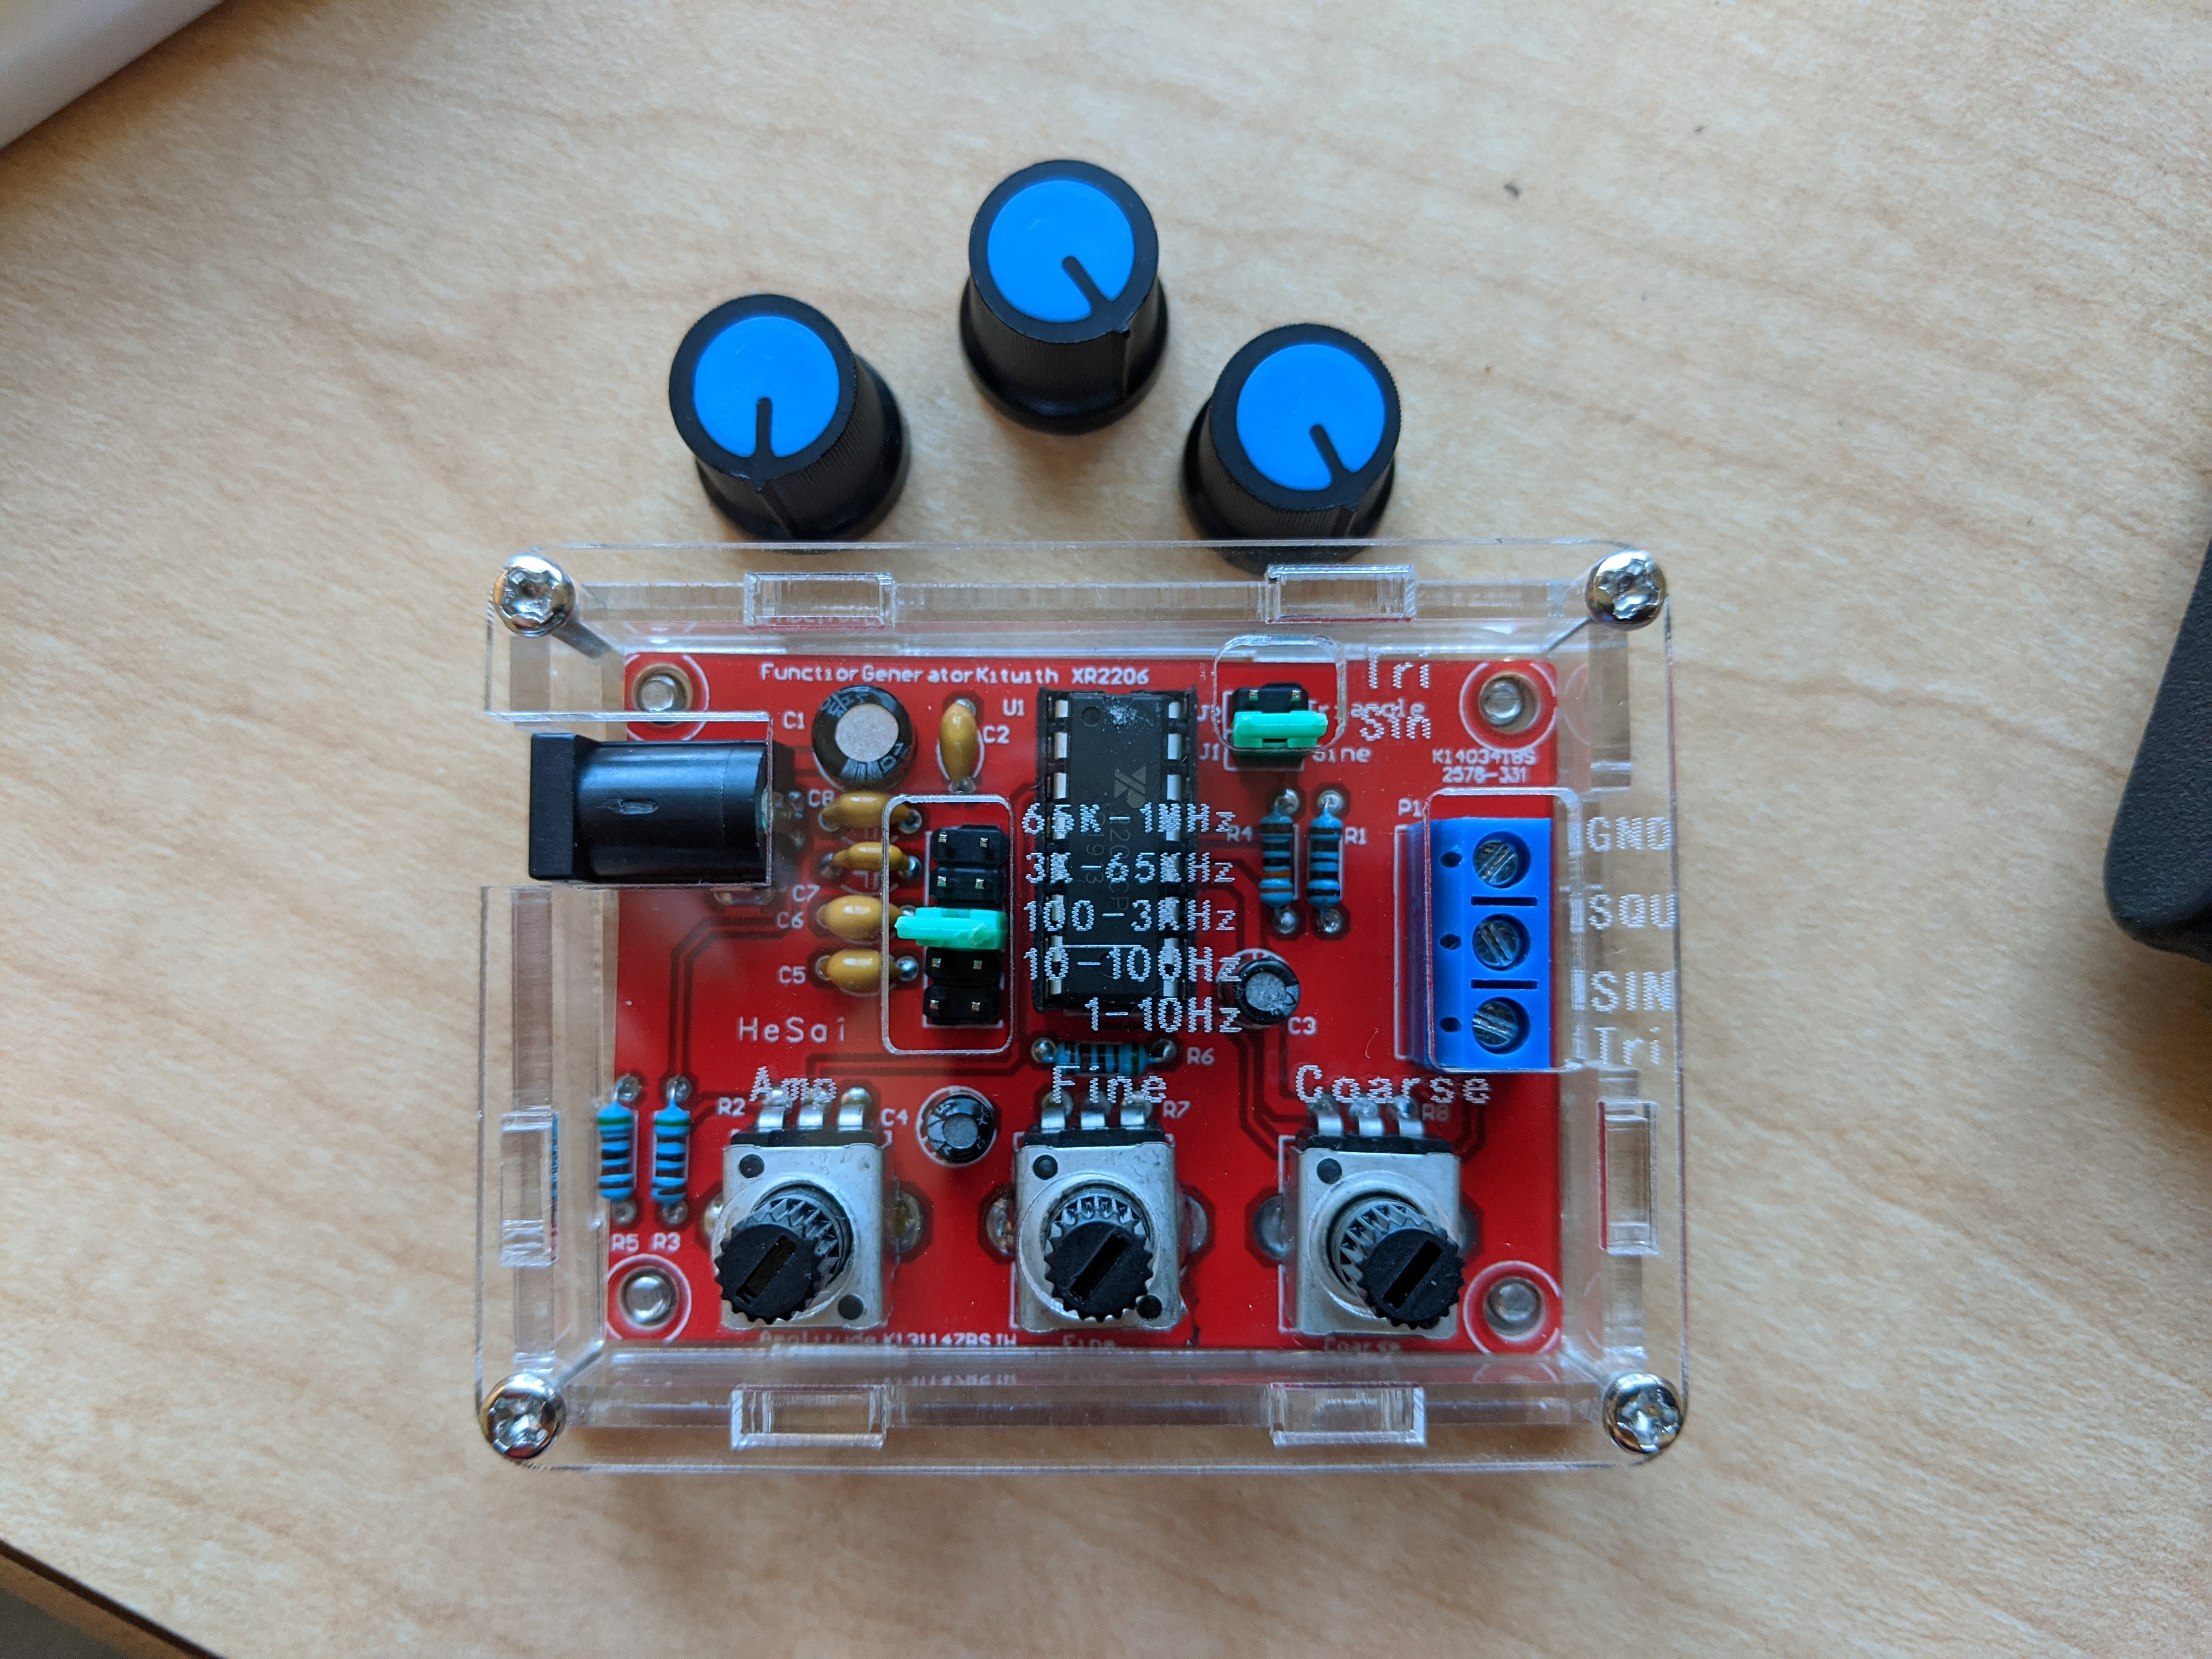
\includegraphics[width=0.78\textwidth]{front.jpg}\par\vspace{1cm}
    \vfill
    
    {\large 
    Written by Astrid Yu\par
    \today}
\end{titlepage}

\section*{Introduction}

The purpose of this experiment is to learn about the soldering and desoldering of electronic components,
both through-hole and surface-mount, as well as to learn about PCB assembly. This will be done using a 
XR2206 function generator kit. A lead will be desoldered to learn about desoldering methods.

\section*{Analysis}

\subsection*{Arduino code used to test the function generator}
\begin{verbatim}
/*
  Analog input, analog output, serial output

  Reads an analog input pin, maps the result to a range from 0 to 255 and uses
  the result to set the pulse width modulation (PWM) of an output pin.
  Also prints the results to the Serial Monitor.

  The circuit:
  - potentiometer connected to analog pin 0.
    Center pin of the potentiometer goes to the analog pin.
    side pins of the potentiometer go to +5V and ground
  - LED connected from digital pin 9 to ground

  created 29 Dec. 2008
  modified 9 Apr 2012
  by Tom Igoe

  This example code is in the public domain.

  http://www.arduino.cc/en/Tutorial/AnalogInOutSerial
*/

// These constants won't change. They're used to give names to the pins used:
const int analogInPin = A0;  // Analog input pin that the potentiometer is attached to
const int analogOutPin = 9; // Analog output pin that the LED is attached to

int sensorValue = 0;        // value read from the pot
int outputValue = 0;        // value output to the PWM (analog out)

void setup() {
  // initialize serial communications at 9600 bps:
  Serial.begin(9600);
}

void loop() {
  // read the analog in value:
  sensorValue = analogRead(analogInPin);
  // map it to the range of the analog out:
  outputValue = map(sensorValue, 0, 1023, 0, 255);
  // change the analog out value:
  analogWrite(analogOutPin, outputValue);

  // print the results to the Serial Monitor:
  Serial.print("sensor = ");
  Serial.print(sensorValue);
  Serial.print("\t output = ");
  Serial.println(outputValue);

  // wait 2 milliseconds before the next loop for the analog-to-digital
  // converter to settle after the last reading:
  delay(2);
}
\end{verbatim}

\subsection*{Images}

\begin{figure}[H]	
    \centering
    \includegraphics[width=\textwidth]{circuit.jpg} 
    \caption{The circuit used to test the function generator.}
    \label{fig:circuit}
\end{figure}

\begin{figure}[H]	
    \centering
    \includegraphics[width=\textwidth]{breadboard.jpg} 
    \caption{The implementation of the circuit on a breadboard.}
    \label{fig:breadboard}
\end{figure}

\begin{figure}[H]	
    \centering
    \includegraphics[width=\textwidth]{screenshot_3.png} 
    \caption{Output from the Arduino Serial Plotter. The frequency is set to 1-10Hz, and the waveform is set to
    triangle. The frequency control is being increased.}
    \label{fig:plotfreq}
\end{figure}

\begin{figure}[H]	
    \centering
    \includegraphics[width=\textwidth]{screenshot_4.png} 
    \caption{Output from the Arduino Serial Plotter. The frequency is set to 1-10Hz, and the waveform is set to
    triangle. The amplitude control is being increased, but the wave appears to be saturating.}
    \label{fig:plotamp}
\end{figure}

\begin{figure}[H]	
    \centering
    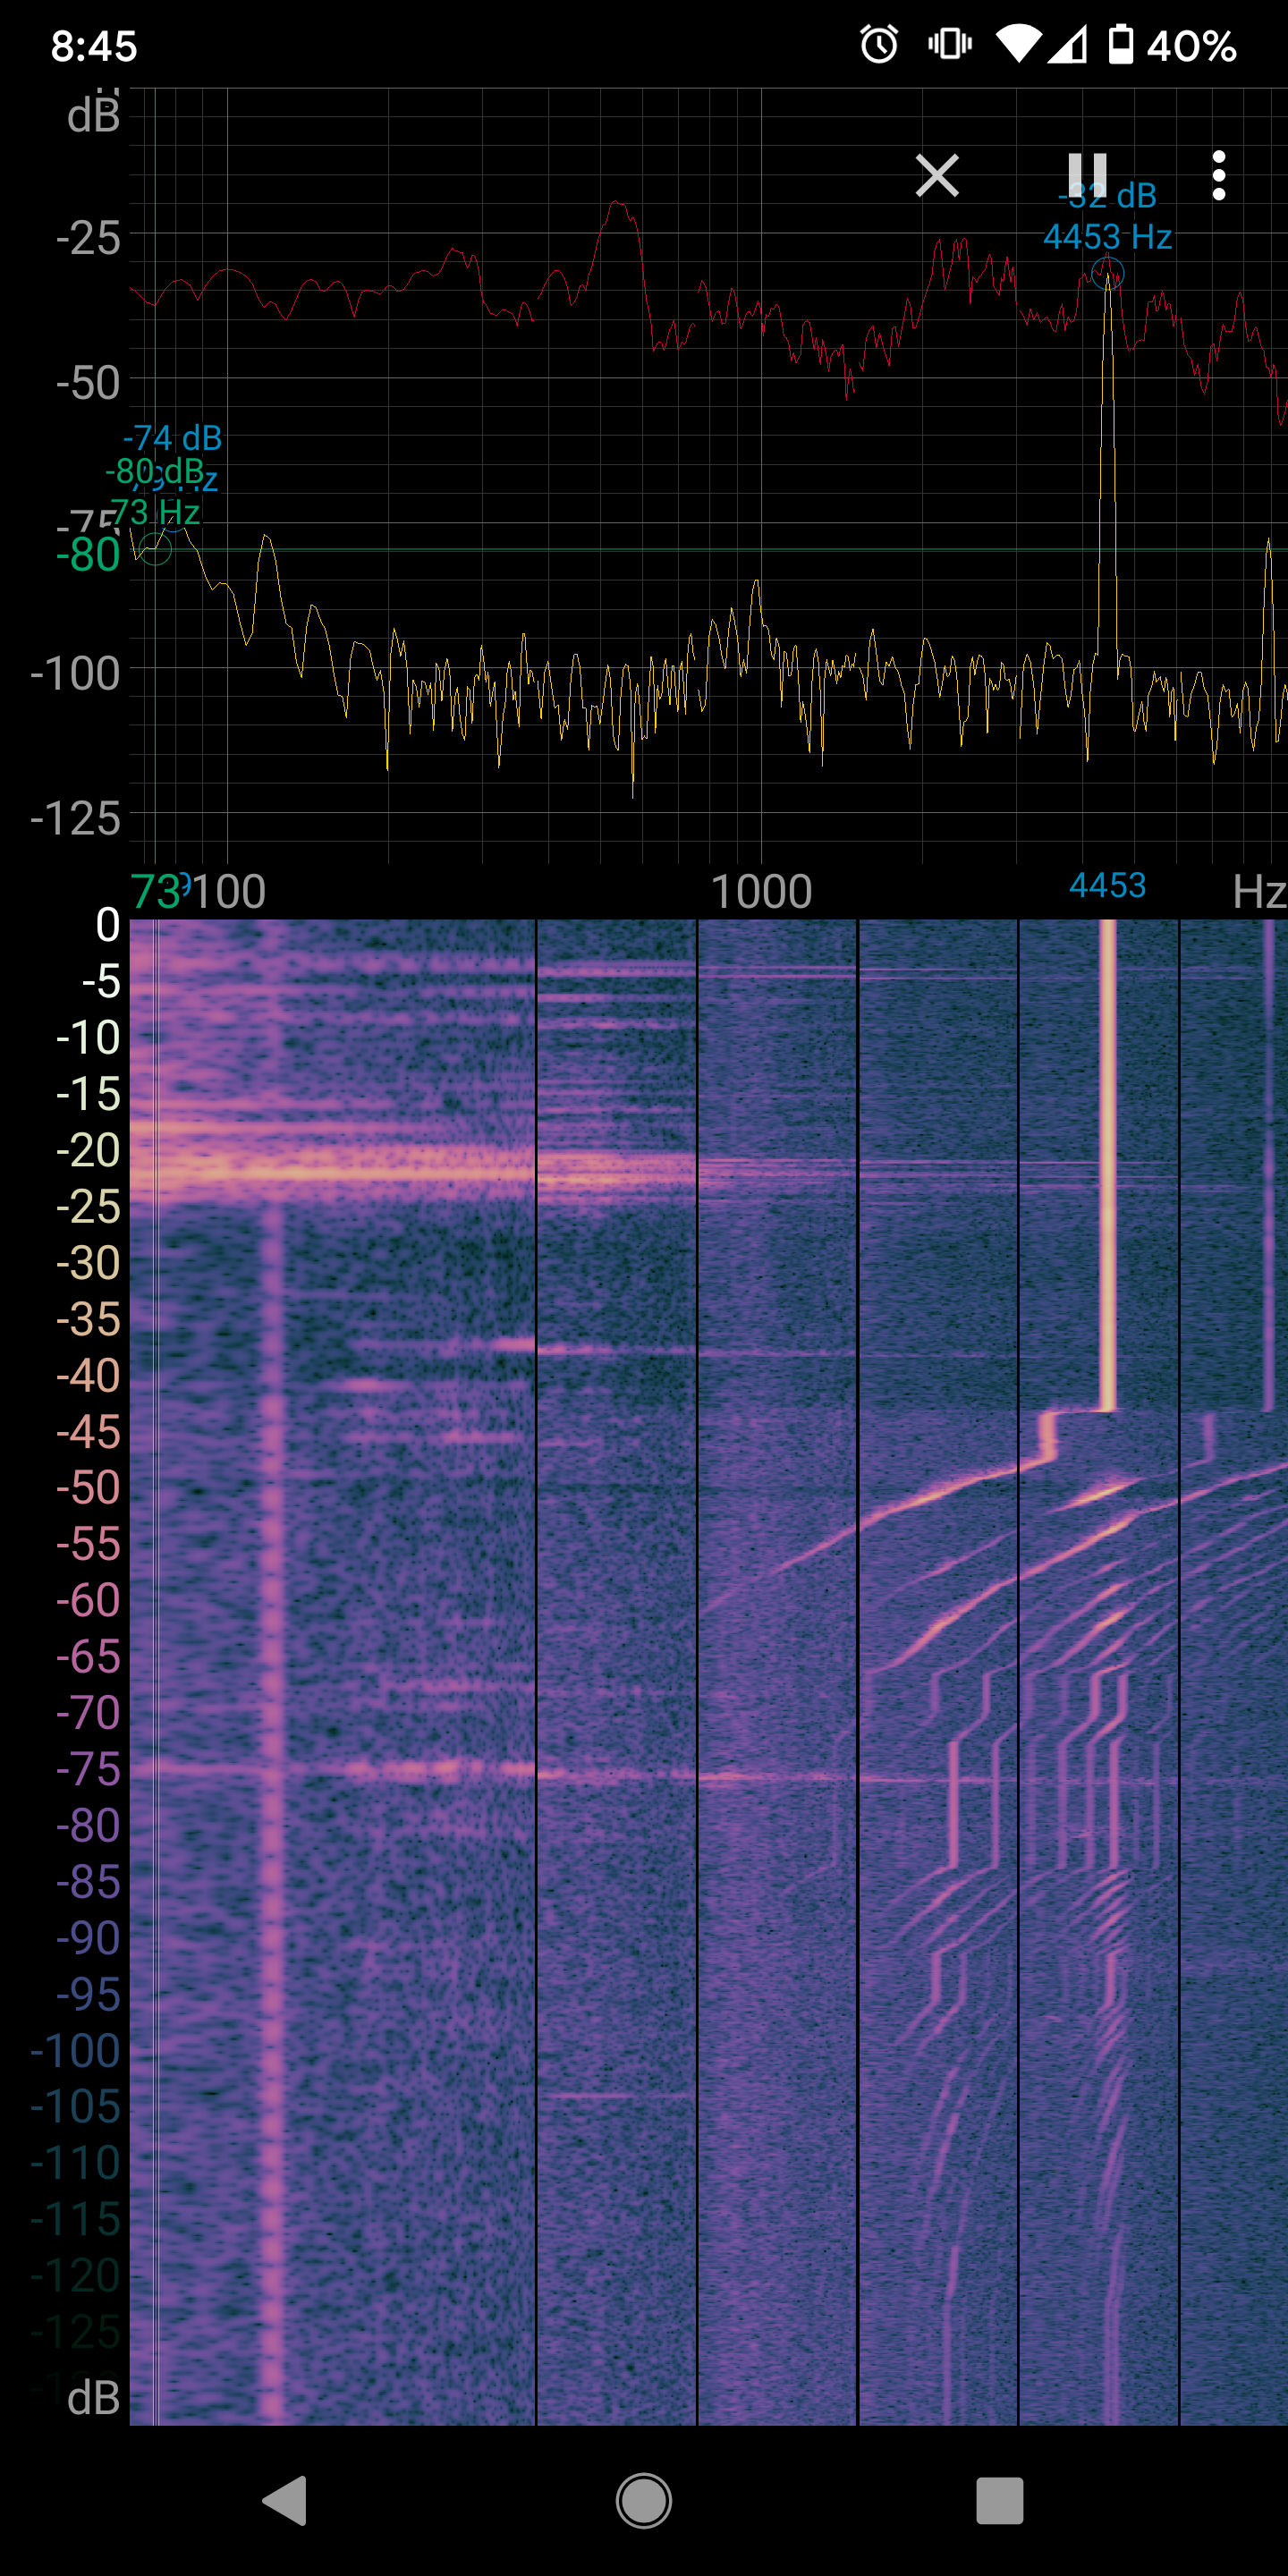
\includegraphics[width=0.5\textwidth]{spec1.png} 
    \caption{Spectrogram of the audio produced by the piezo connected to the transistor. The frequency is 
    set to 100-3KHz, and the waveform is a square wave. The frequency was being increased until it reached
    the maximum frequency of 4453 Hz. However, the response of the spectrogram is seen to be fading out 
    towards the lower ranges, so a measurement for the minimum frequency could not be made.}
    \label{fig:speca}
\end{figure}

\begin{figure}[H]	
    \centering
    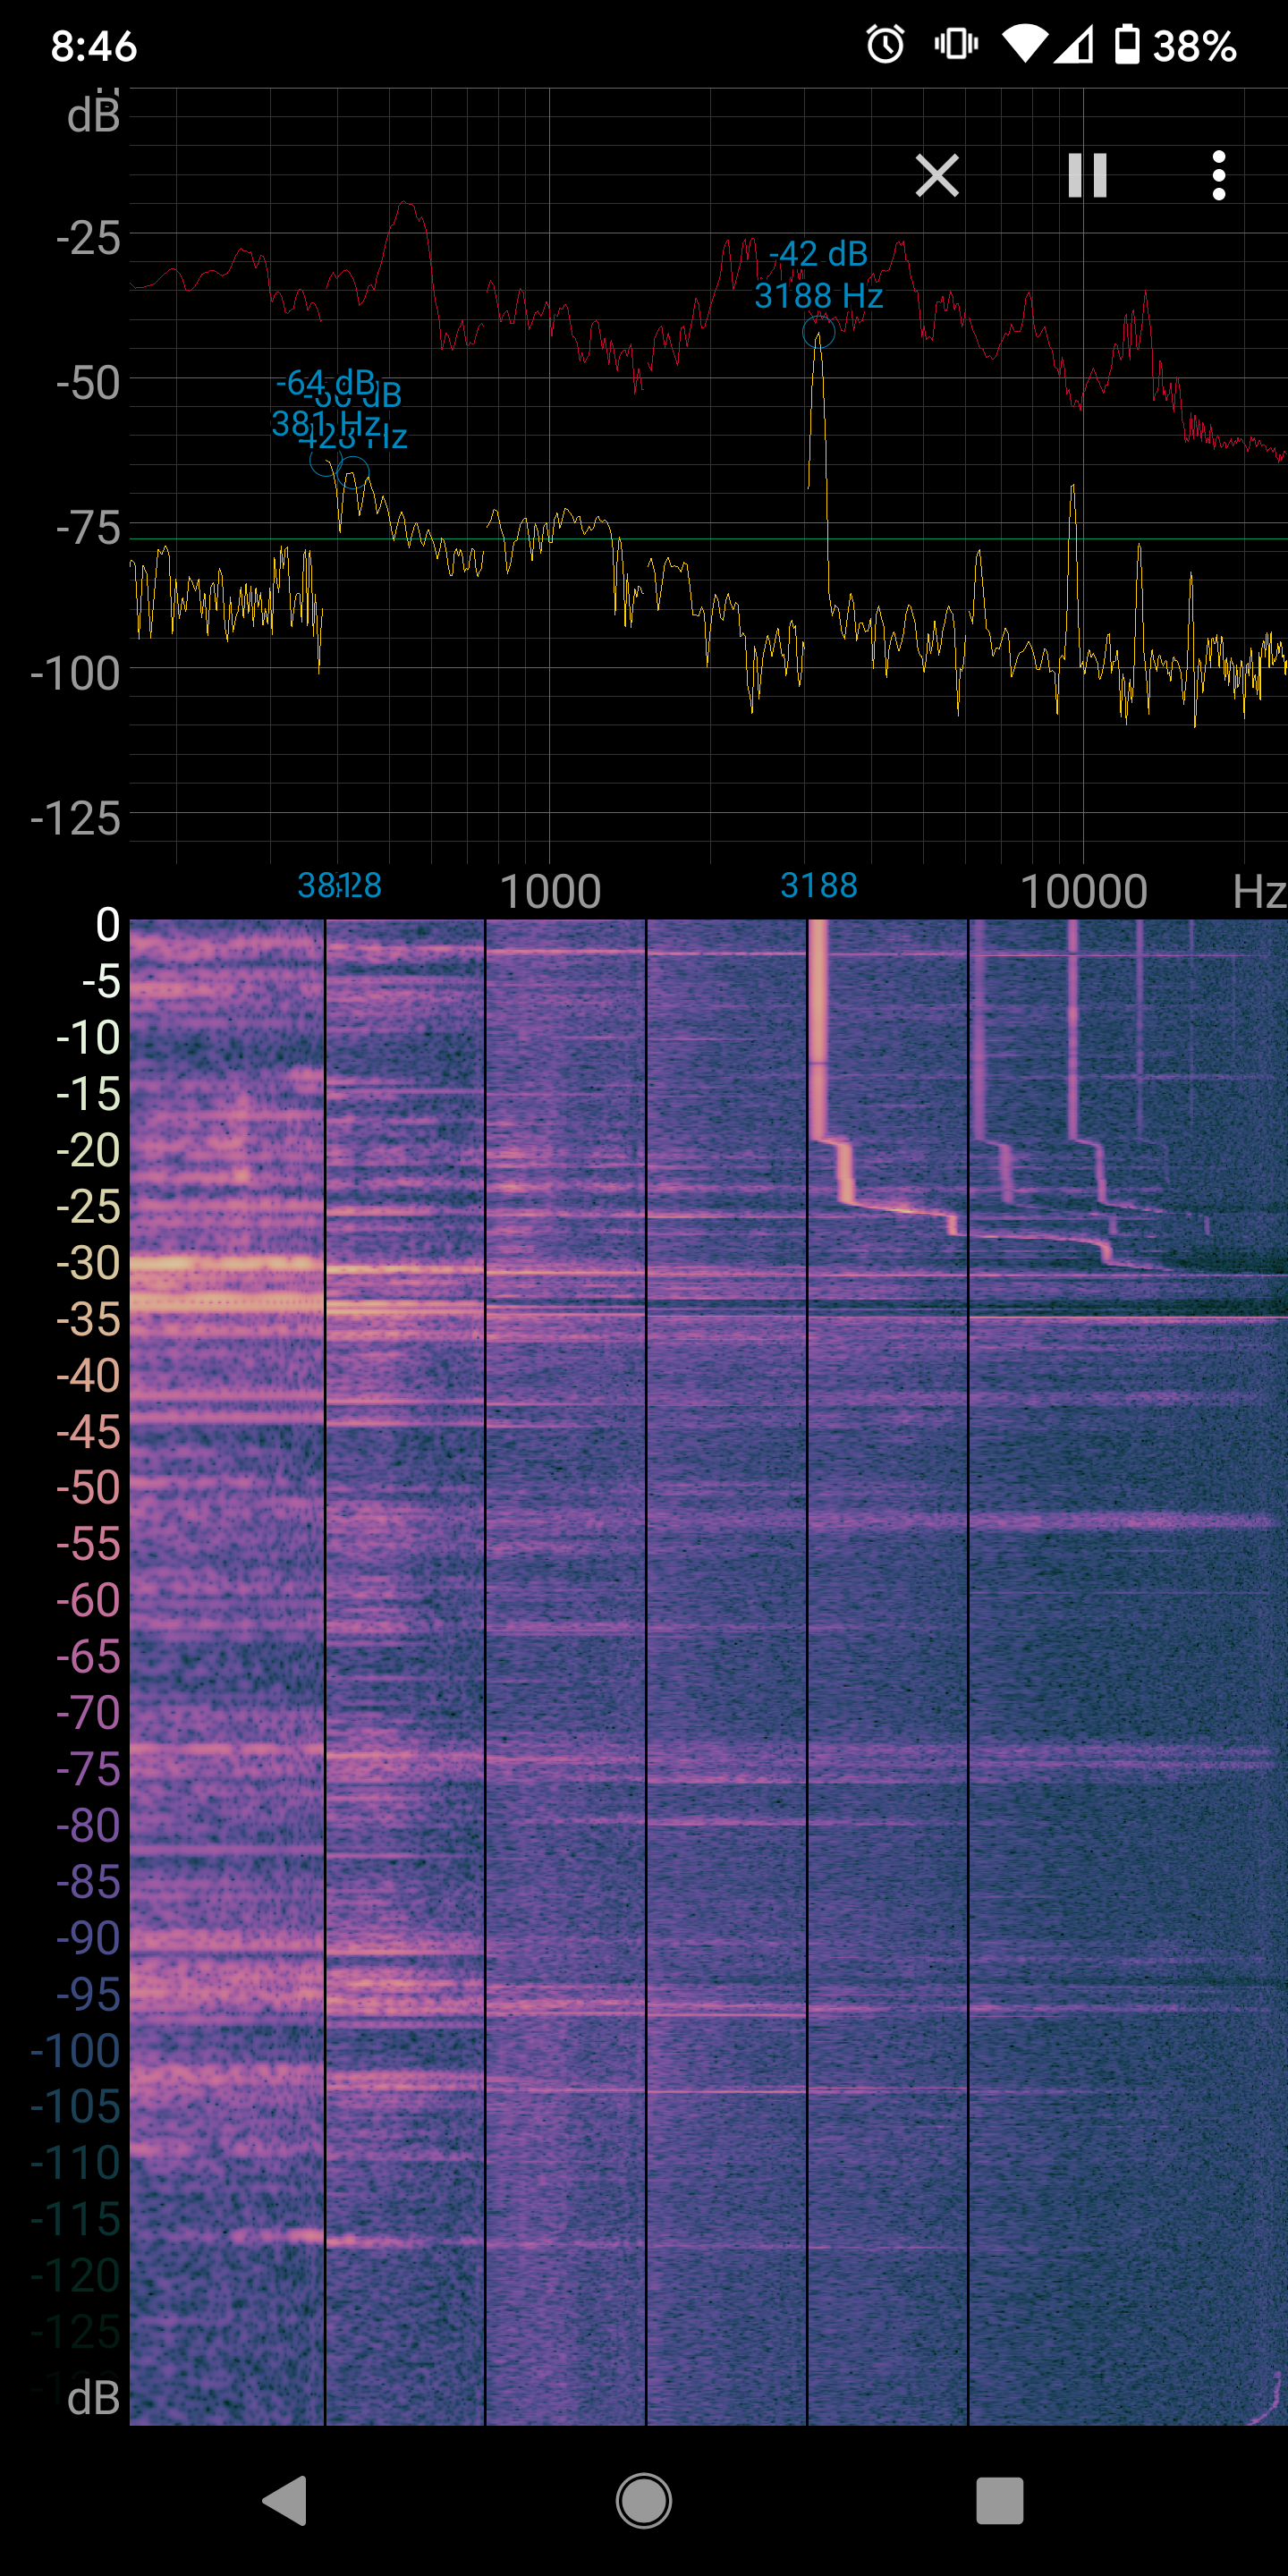
\includegraphics[width=0.5\textwidth]{spec3.png} 
    \caption{Spectrogram of the audio produced by the piezo connected to the transistor. The frequency is 
    set to 3K-65KHz, and the waveform is a square wave. The minimum frequency is capping out at 3188 Hz.}
    \label{fig:specb}
\end{figure}

\begin{figure}[H]	
    \centering
    \includegraphics[width=0.5\textwidth]{spec4.png} 
    \caption{Spectrogram of the audio produced by the piezo connected to the transistor. The frequency is 
    set to 3K-65KHz, and the waveform is a square wave. The frequency is being increased until it exceeds 
    the limits of the spectrogram (maximum 20KHz).}
    \label{fig:specc}
\end{figure}

\section*{Discussion}

\subsection*{1. Soldering}
\begin{enumerate}
    \item {
        \textit{What do you consider to be the most challenging aspect of soldering?}

        The most challenging aspect of soldering is the soldering of SMD parts because of the precision
        and control needed. The function generator kit did not have any SMD parts to solder, but the difficulty
        of SMD soldering is known from a project from the past.
    } 
    \item {
        \textit{Why is it likely your project will not work even if one solder joint is ``cold'' (not shiny and smooth, but dull and crumbly)?}

        Cold joints are poor joints that do not create a mechanically strong electrical path between the lead and the trace. This can introduce resistance,
        and in some cases, it may not even be properly connected.

        In a circuit like the function generator kit, there is an oscillator. Its frequency could be sensitive to small changes in resistance because that can 
        affect the rate of charge buildup in the capacitors, or magnetic field buildup in the inductors.
    }  
    \item {
        \textit{What is the practical reason to assemble components flush to the board?}
        
        Assembling components flush to the board makes the entire circuit take up less volume. Additionally, when the component is not flush,
        the leads would be more exposed, and the part is more vulnerable to mechanical damage and oxidation.
    }  
    \item {
        \textit{Take close-up pictures of the component side and trace side of your project PCB, insert here.}
       
        \centering

        \includegraphics[width=0.45\textwidth]{fr2.jpg}
        \includegraphics[width=0.45\textwidth]{rear.jpg}
    }
    \item {
        \textit{Did you have to troubleshoot your project? If so, were you successful in finding the problem?}
        
        Some troubleshooting was necessary, but the board did not need any modification At first, a 6V AA battery
        array was supplied to the the function generator. However, no waveform output was observed because 
        the circuit needed a 9V supply. When the 9V battery was connected, however, a waveform was observed.
    }   
\end{enumerate}

\subsection*{2. Desoldering}
\begin{enumerate}
    \setcounter{enumi}{6} 
    \item {
        \textit{What do you consider the most challenging aspect of de-soldering to be?}

        The most challenging aspect of desoldering is removing parts with many pins. Header pins and ICs 
        are the most challenging ones to remove because if even one pin does not have all the solder removed 
        from it, the entire component will be anchored in place by that one pin.
    } 
\end{enumerate}


\section*{Conclusion}

The assembly of the function generator was very successful. The function generator did not need any 
fixes after it was initially assembled. Additionally, desoldering a resistor was successful, and copper 
traces were not damaged in the process.

Testing the functionality and capabilities of the function generator was also successful. On the lowest frequency step, an output was 
detected as seen in Figures \ref{fig:plotfreq} and \ref{fig:plotamp}. However, a limitation of the part
was also found; it saturates very easily at high amplitude settings as evidenced by Figure \ref{fig:plotamp}.

The upper limit of the 100Hz-3kHz step was successfully established using a spectrogram.
The limit was found to be 4453 Hz (Figure \ref{fig:speca}), which is past 3kHz. This is good, because it demonstrates that every frequency advertised 
is included. However, the lower limit could not be established because the piezo 
appears to have a very poor frequency response for frequencies below the kHz range, as shown in the figure.

The minimum limit of the 3kHz-65kHz step was also established, and found to be 3188 kHz (see Figure \ref{fig:specb}).
This does not include the advertised 3kHz frequency, so if a 3kHz frequency is required, the 100Hz-3kHz step 
should be used. Due to the limitations of the spectrogram app and the piezo, the upper limit was not able to be established (see Figure \ref{fig:specc}).

\end{document}